\documentclass[12pt,a4paper,oneside]{report}
\usepackage[utf8x]{inputenc}
\usepackage[english]{babel}
\usepackage[top=2.5cm, bottom=3cm, left=2.5cm, right=2.5cm, bindingoffset=0.5cm]{geometry}
\usepackage{graphicx}

\graphicspath{{./pics/}}

\usepackage{hyperref}
\hypersetup{hidelinks=true}
\hypersetup{pdftitle={HANS - BMEGT43A066 Report}}
\hypersetup{pdfauthor={Richárd József Beregi \& Tamás Lévai}}

\begin{document}

\begin{titlepage}
{ \center \resizebox{11cm}{!}{
\includegraphics{bme_logo_nagy.jpg}}
\vspace{0.5cm}

{\large \bf Budapest University of Technology and Economics} \\[10pt]
\vfill
{\Large Richárd József Beregi \& Tamás Lévai} \\[20pt]
{\LARGE HANS} \\[20pt]
{\Large Report for Recorded Music} \\[20pt]
\vfill
{\bf Supervisor}:\\[20pt]

Dr. Emília Barna
\vfill
{\Large Budapest, 2015.}

}
\end{titlepage}

\section*{Introduction}

\subsection*{Concept}
Our base idea was to involve the computer as an autonomous entity in a
musical band. This is a progressive idea, because involving non-human
actors into creative works is still not common in the western
culture. Artistic works in the past presented the intelligent,
autonomic machines as dangerous entities which should be
avoid. Nowadays, this attitude seems shifting. There are various
artistic performances -- mainly in the field of conceptual art --
incorporating autonomic computers as a media. A great musical example
of this phenomena is netcat, a band of two cellist, a synthesizer
player and three computers.

There are various ways to create sounds with a computer. Our approach
was to tread tread the computer as a sampler guy. We gave it a large
number of audio files and access to its environment: it can listen to
other musicians or even see the surroundings. Based on these inputs it
will be able to choose samples corresponding to the music.

\subsection*{HANS}
We implemented our concept as a software using the Pyo~\footnote{Pyo
  website: {\small \url{http://ajaxsoundstudio.com/software/pyo/}}}
audio library. Pyo is a Python-based framework for programming signal
processors and synthesizers. We named the software HANS. This name
reflects to the common German name, Hans, and it is also the acronym
of Human-like Audio Network System.

In the context of the homework we implemented the proof-of-concept of
our idea. We tried to focus on the experimental noise punk genre,
therefore, this version is capable to play out random samples randomly
at beats.  To achieve this functionality, the program consist of
multiple building blocks. The main building block is the Modulator
which randomly plays out the random samples. These samples are
provided by the Chooser which is responsible to select samples from a
local directory that is full of sample files. Chooser's selection is
controlled by SeedGen. SeedGen can provide a random seed for Chooser
from many sources (e.g., webcam image, network traffic). Currently, it
only supports the pseudo-random generator of Python. Beside sample
choosing, the program has one more important aspect: timing. It was a
design choice that the samples should be played when a beat occurs. To
detect beats we connected the drum via MIDI and declared the accented
bass drum as a beat (in MIDI this is translated as status 153 with
note 36 and a velocity greater than 48). For detecting beats on MIDI
input, the MidiProc block is responsible.

The program can run on various operating systems and audio
systems. During the demonstration we used Debian GNU/Linux with the
low-latency JACK~\footnote{JACK website: {\small
    \url{http://www.jackaudio.org/}}} audio system. In
Figure~\ref{fig:hans_screen} you can see a snapshot from the
demonstration. On the top-right corner there is the JACK controller
program, on the left there is the source code of HANS, and on the
top-left there is the graphical user interface of HANS.

\begin{figure}[h!]
\centering
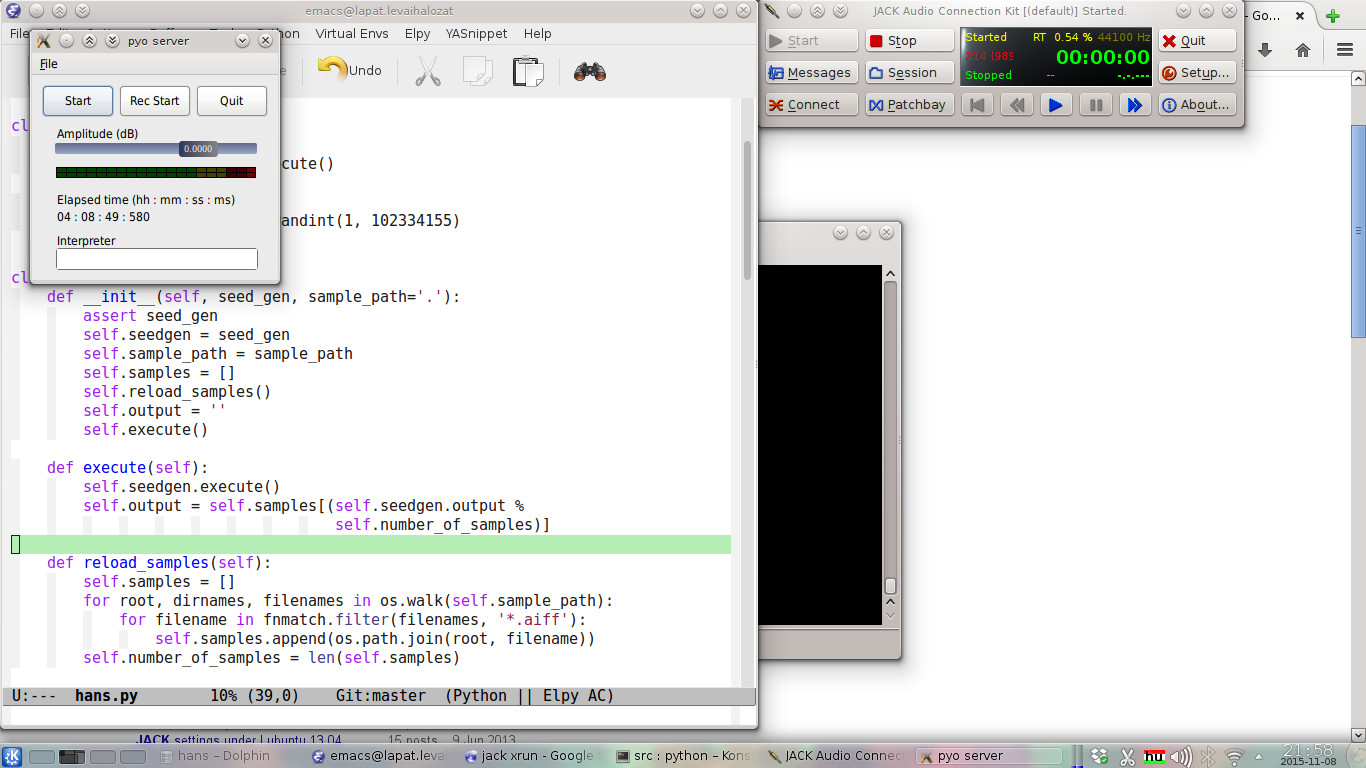
\includegraphics[width=0.7\textwidth]{snapshot.jpg}
\caption{Snapshot of HANS}
\label{fig:hans_screen}
\end{figure}

\section*{First Session: Demonstrating HANS}

\subsection*{Recording Environment}
Our first jam session with the proof-of-concept version of HANS took
place at Richárd Beregi's flat on a cosy Sunday evening in November
2015 (It wasn't a dark and stormy night). Since all of our instruments were electronic, there was no real
need to go to a studio with great acoustics, so we just wired up all of
our devices into an analogue mixer, hooked a recorder and put our
headphones on in a common living room as you can see in
Figure~\ref{fig:rec_env}.

\begin{figure}[h!]
\centering
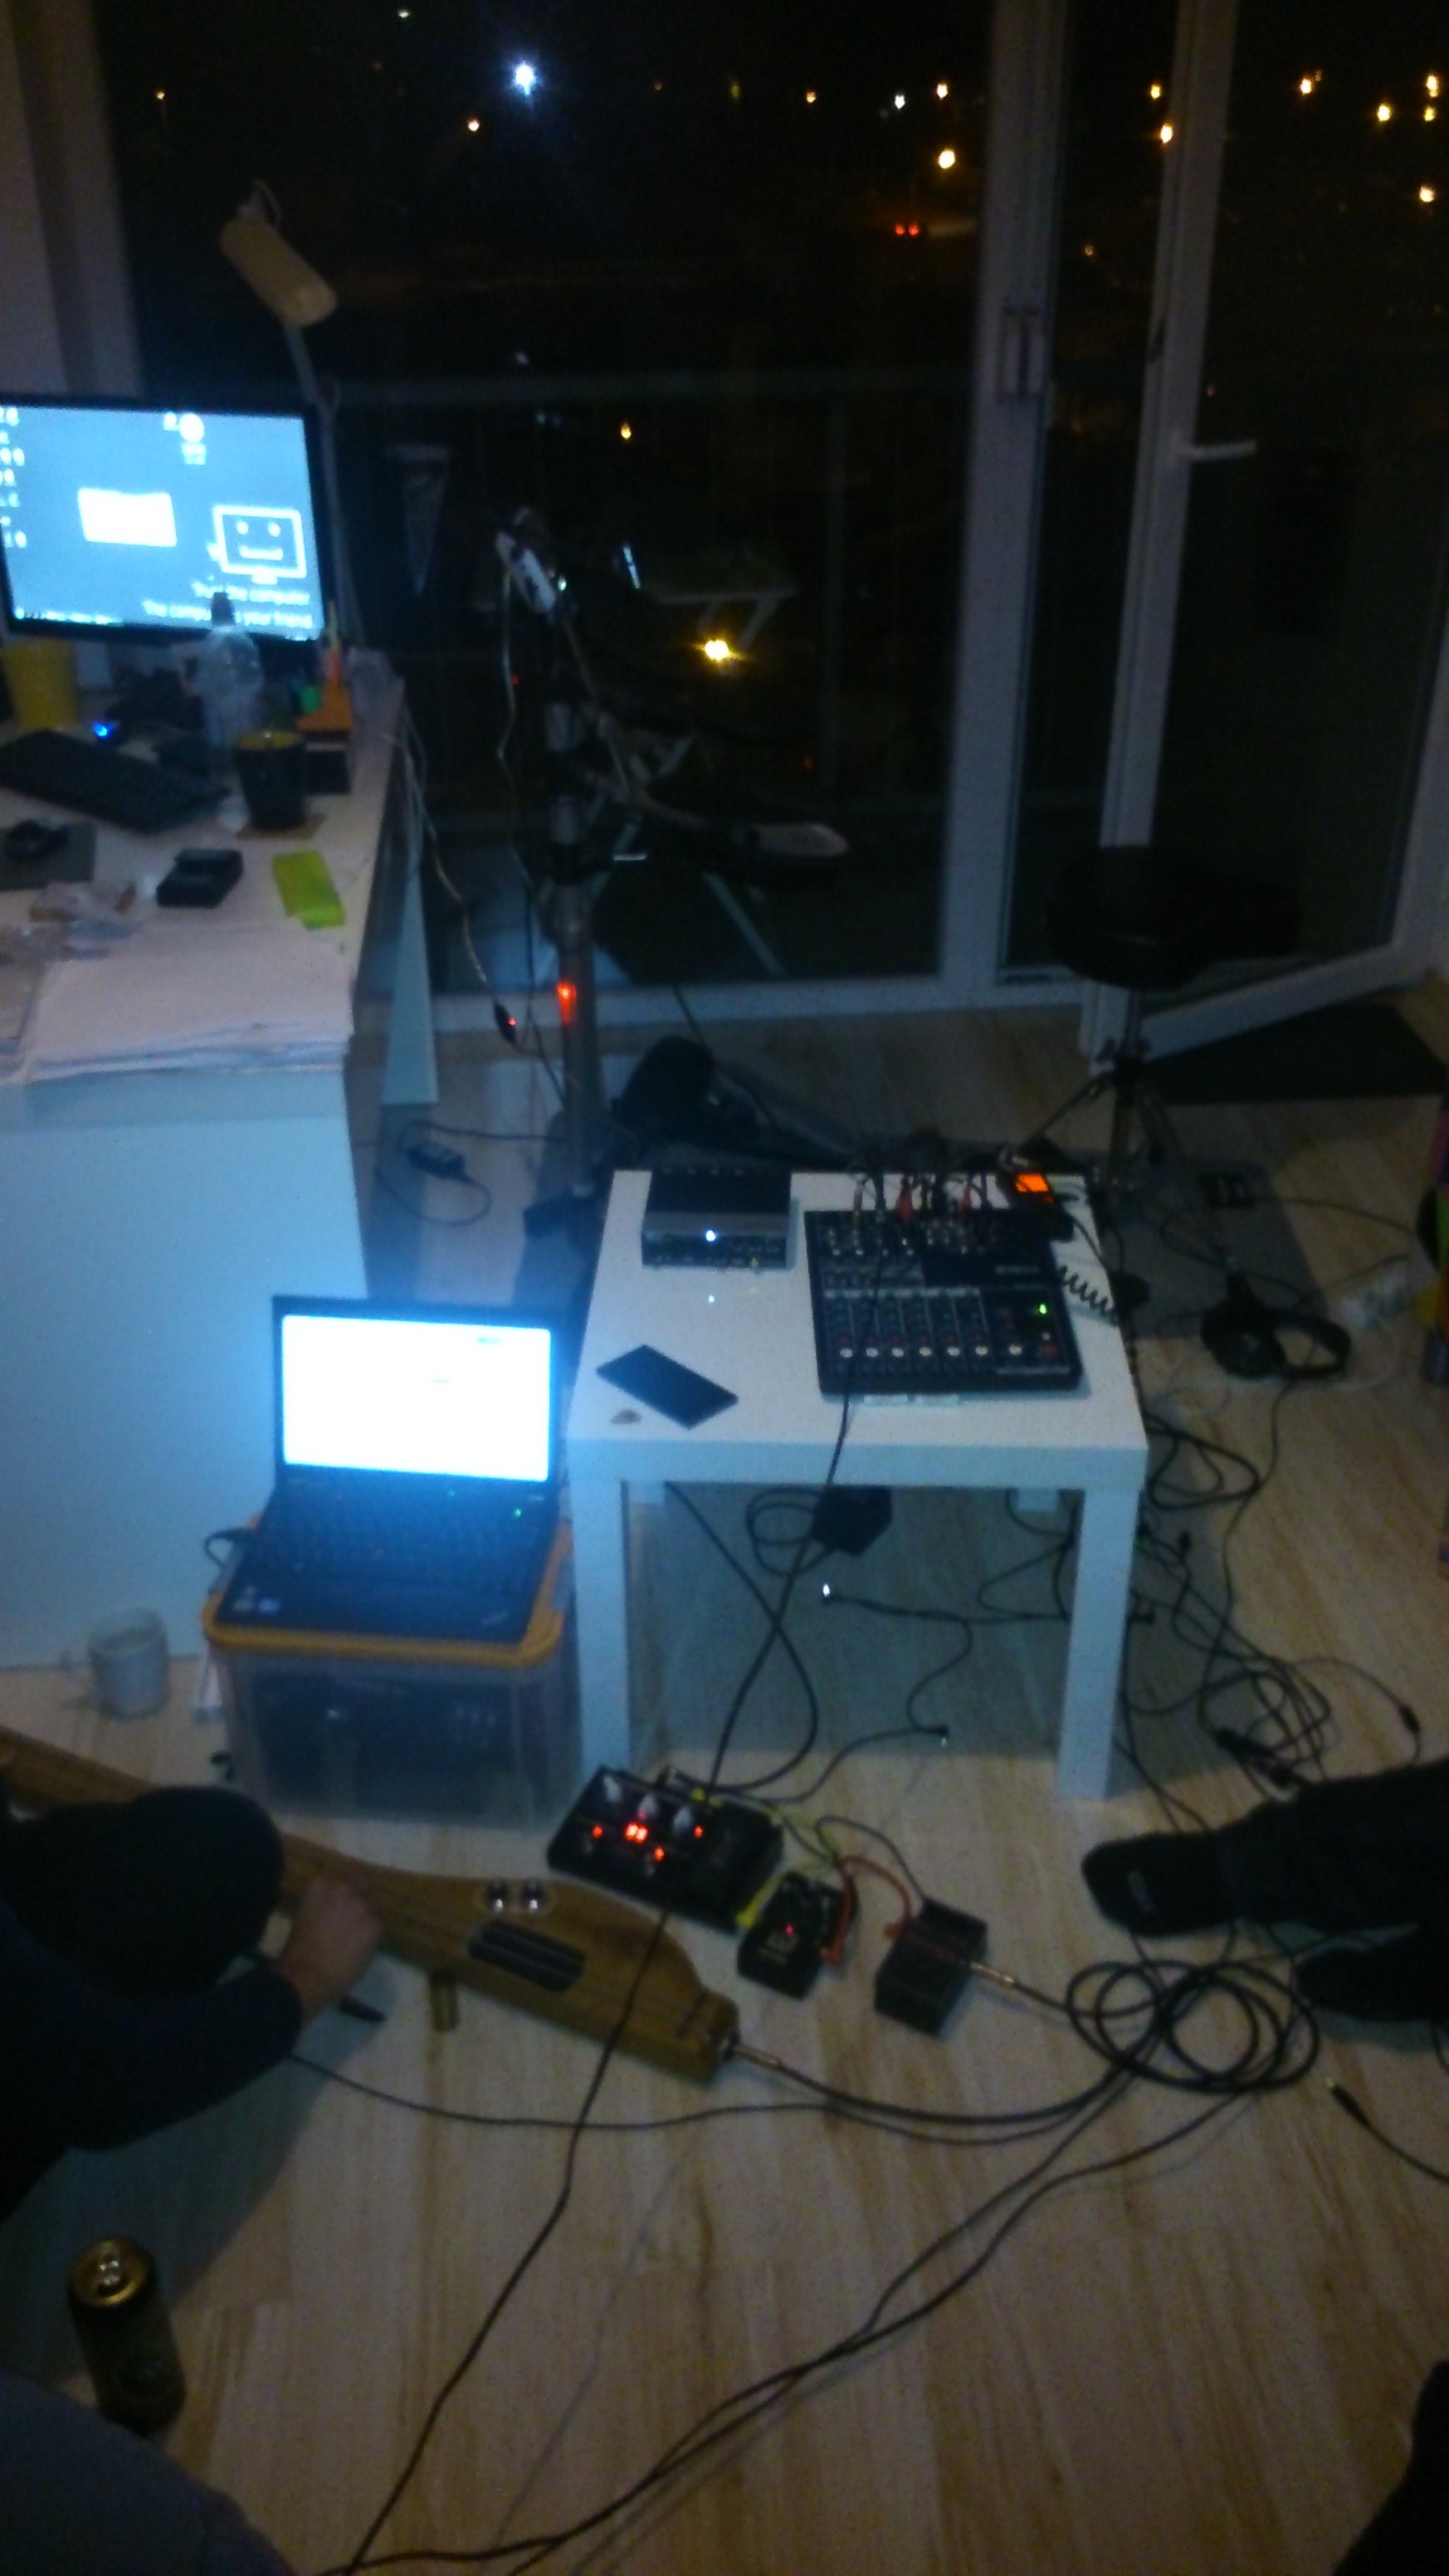
\includegraphics[width=0.45\textwidth]{DSC_0402.jpg}
\caption{The Recording Environment}
\label{fig:rec_env}
\end{figure}

The set-up of the instruments worth further explanation due to its
complexity. HANS was running on a computer with an external sound
card. The stereo audio output of the sound card was directly connected
to the analogue mixer, and the electronic drum was connected to its
MIDI input. Unfortunately, we had no MIDI cable at that time, so we
used an other computer with a different operating system and an
USB-MIDI converter to transfer MIDI signals from the electronic drum
to the computer running HANS. In parallel, the audio output of the
drum was connected to the mixer. With this twisted set-up we were able
to control HANS and to hear the drum sound. The synthesizers, a Korg
Monotron Delay and a Korg Mini Kaoss Pad 2, were either directly
connected to the mixer or daisy-chained. The last instrument, the so
called home-made \emph{electric bass-zither}, was connected to the
mixer via an effect chain.

During the session, Richárd Beregi played the drums, Tamás Lévai played
the electric bass-zither. Guest participants, Tamás Kristóf and Gábor
Bényei played the synthesizers. The recorder was managed by Gábor
Bényei.

\subsection*{Recording}
\label{ss:recording}
The target of our first session was to create a demonstration of HANS
in the genre of experimental noise punk. Therefore, we recorded the
whole session (three and a half hour long) and chose the right part of
it, however, that was not an easy task; during the session large
amount of time was spent for rehearsing purposes; an other significant
amount of the recording was noisy drone with no sign of
HANS. Obviously, these parts were not able to demonstrate HANS
well. Finally, we chose a 15 minutes continuous excerpt as a
demonstration to share. This excerpt contains every important aspect
of the first session: the samples played by HANS and the distorted
electric-bass zither sound decorated with some synthesizer sounds in
an improvised manner creates a noisy, ever changing atmosphere which
never rests.

\subsection*{Cover Art}
Every musical composition needs a visualisation which delivers the
concept and the core of the music at first look. Our approach for this
can be seen in Figure~\ref{fig:cover_art}. The colorization and the
chaoticness are in accordance with the experimental noise punk
genre. The neon contours of every cable are multiplied with an fractal
algorithm, which is a method commonly associated with computer
science. Even the most noticeable fragments of the figure are the
computer screens. The background story of the base picture (taken
during the first session in Richárd's flat) just an extra feature,
that we can disregard. We can say that the creator wanted to tell us
something with the duplicated and turned upside-down half of the
figure, but in reality we just wanted to make it in a square form and
this was the easiest, yet most artistic way. We added the 'HANS' label
to assign it with the music. The photo was taken with a smart phone,
while it was edited with GNU Image Manipulation Program (GIMP 2.0).


\begin{figure}[h!]
\centering
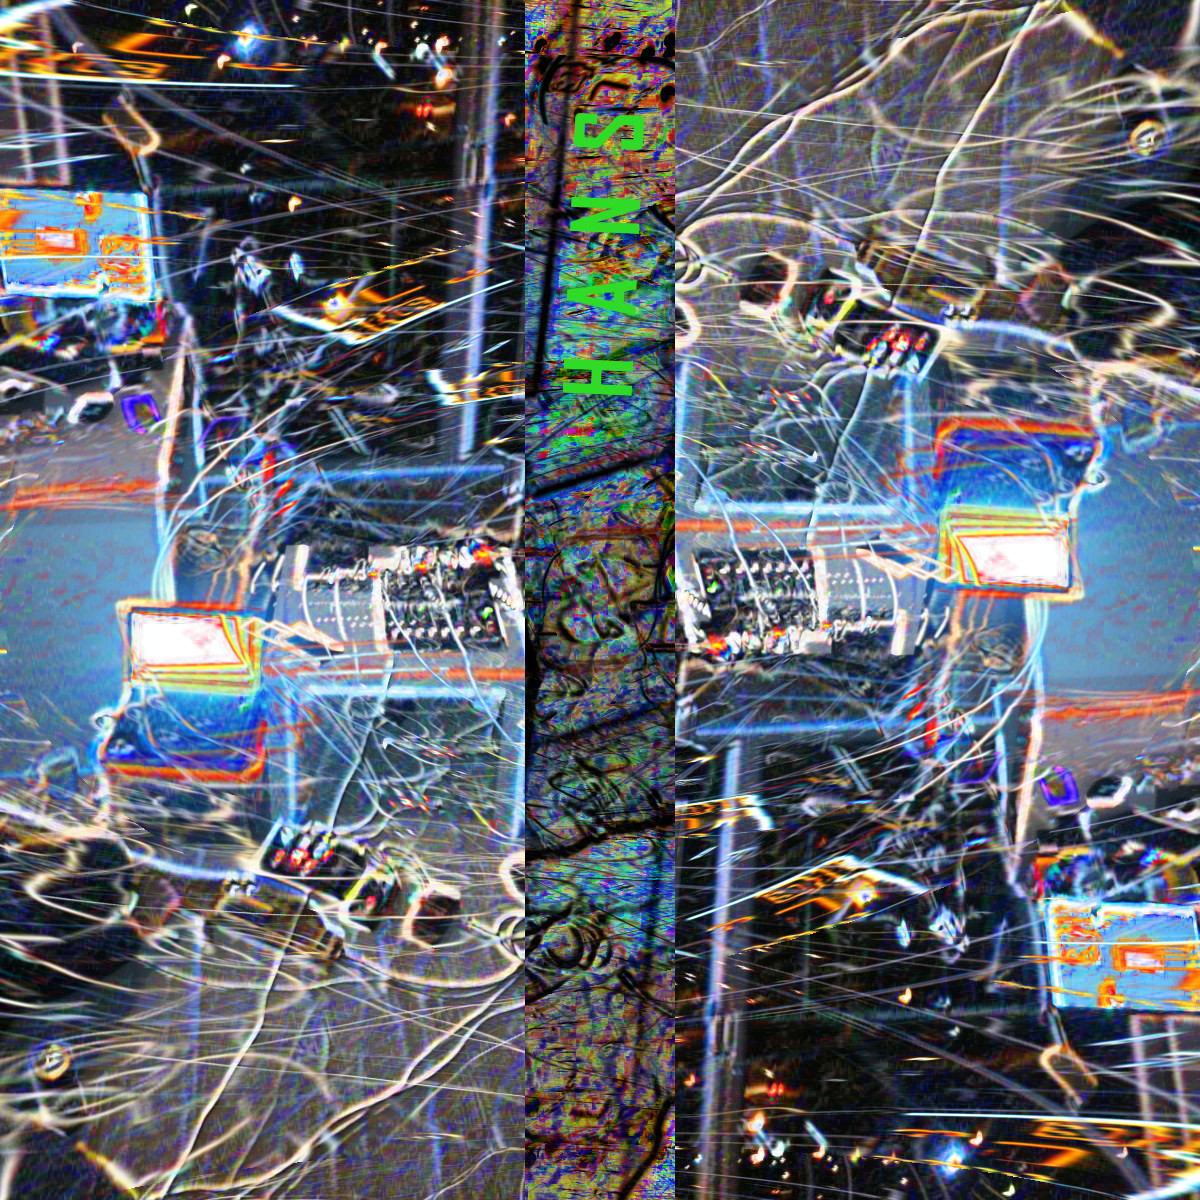
\includegraphics[width=0.6\textwidth]{hans_neon_1x2.jpg}
\caption{The Cover Art}
\label{fig:cover_art}
\end{figure}

\subsection*{Distribution}
The recording mentioned in Section~\ref{ss:recording} was uploaded to
public sound-sharing site, Soundcloud. The recording can be listened
and commented by anyone on the following URL:
\url{https://soundcloud.com/leait/hans-0000001}.

\subsection*{Feedback}
We tried to get as much feedback as possible from the uploaded
recording, therefore, we sent the link to many of our friends.  Their
responses were the following:

\begin{itemize}
\item ``The music of HANS is awesome to get home after heavy drinking.''
\item ``I can not process the experience.''
\item ``I listened to it fully only once. Not any more.''
\end{itemize}

\section*{Summary}
\subsection*{Conclusion}
In this project we created an audible piece of conceptual art. One
output of this project is the recording we made and the cover art we
created. The other output is the software on which we can build later.

\subsection*{Future Work}
However, we completed the homework, our project is still far from
finished. Since the software we created is still a proof-of-concept,
we should consider its improvement in the near future (i.e., involving
the reflections of the computer's environment into sample choosing at
real-time). Beside the improvement of the software, we are considering
to arrange rehearsals and performances, involving other musicians,
etc.

\section*{Acknowledgements}
We would like to express our very great appreciation to Dávid Szabó
for his valuable suggestions and help during the planning of HANS.

We would like to offer our special thanks to Gábor Bényei and Tamás
Kristóf for participating in the first session, and Kinga Kovács and
Gábor Bényei for their samples.

Last but not least, we wish to thank everyone who provided some
feedback or help to this project.
\end{document}